\providecommand{\main}{../../../..}
\documentclass[\main/dresen_thesis.tex]{subfiles}
\begin{document}
  \label{sec:monolayers:nanoparticle:vsm}

  \paragraphNewLine{Vibrating Sample Magnetometry}
    \begin{figure}[tb]
      \centering
      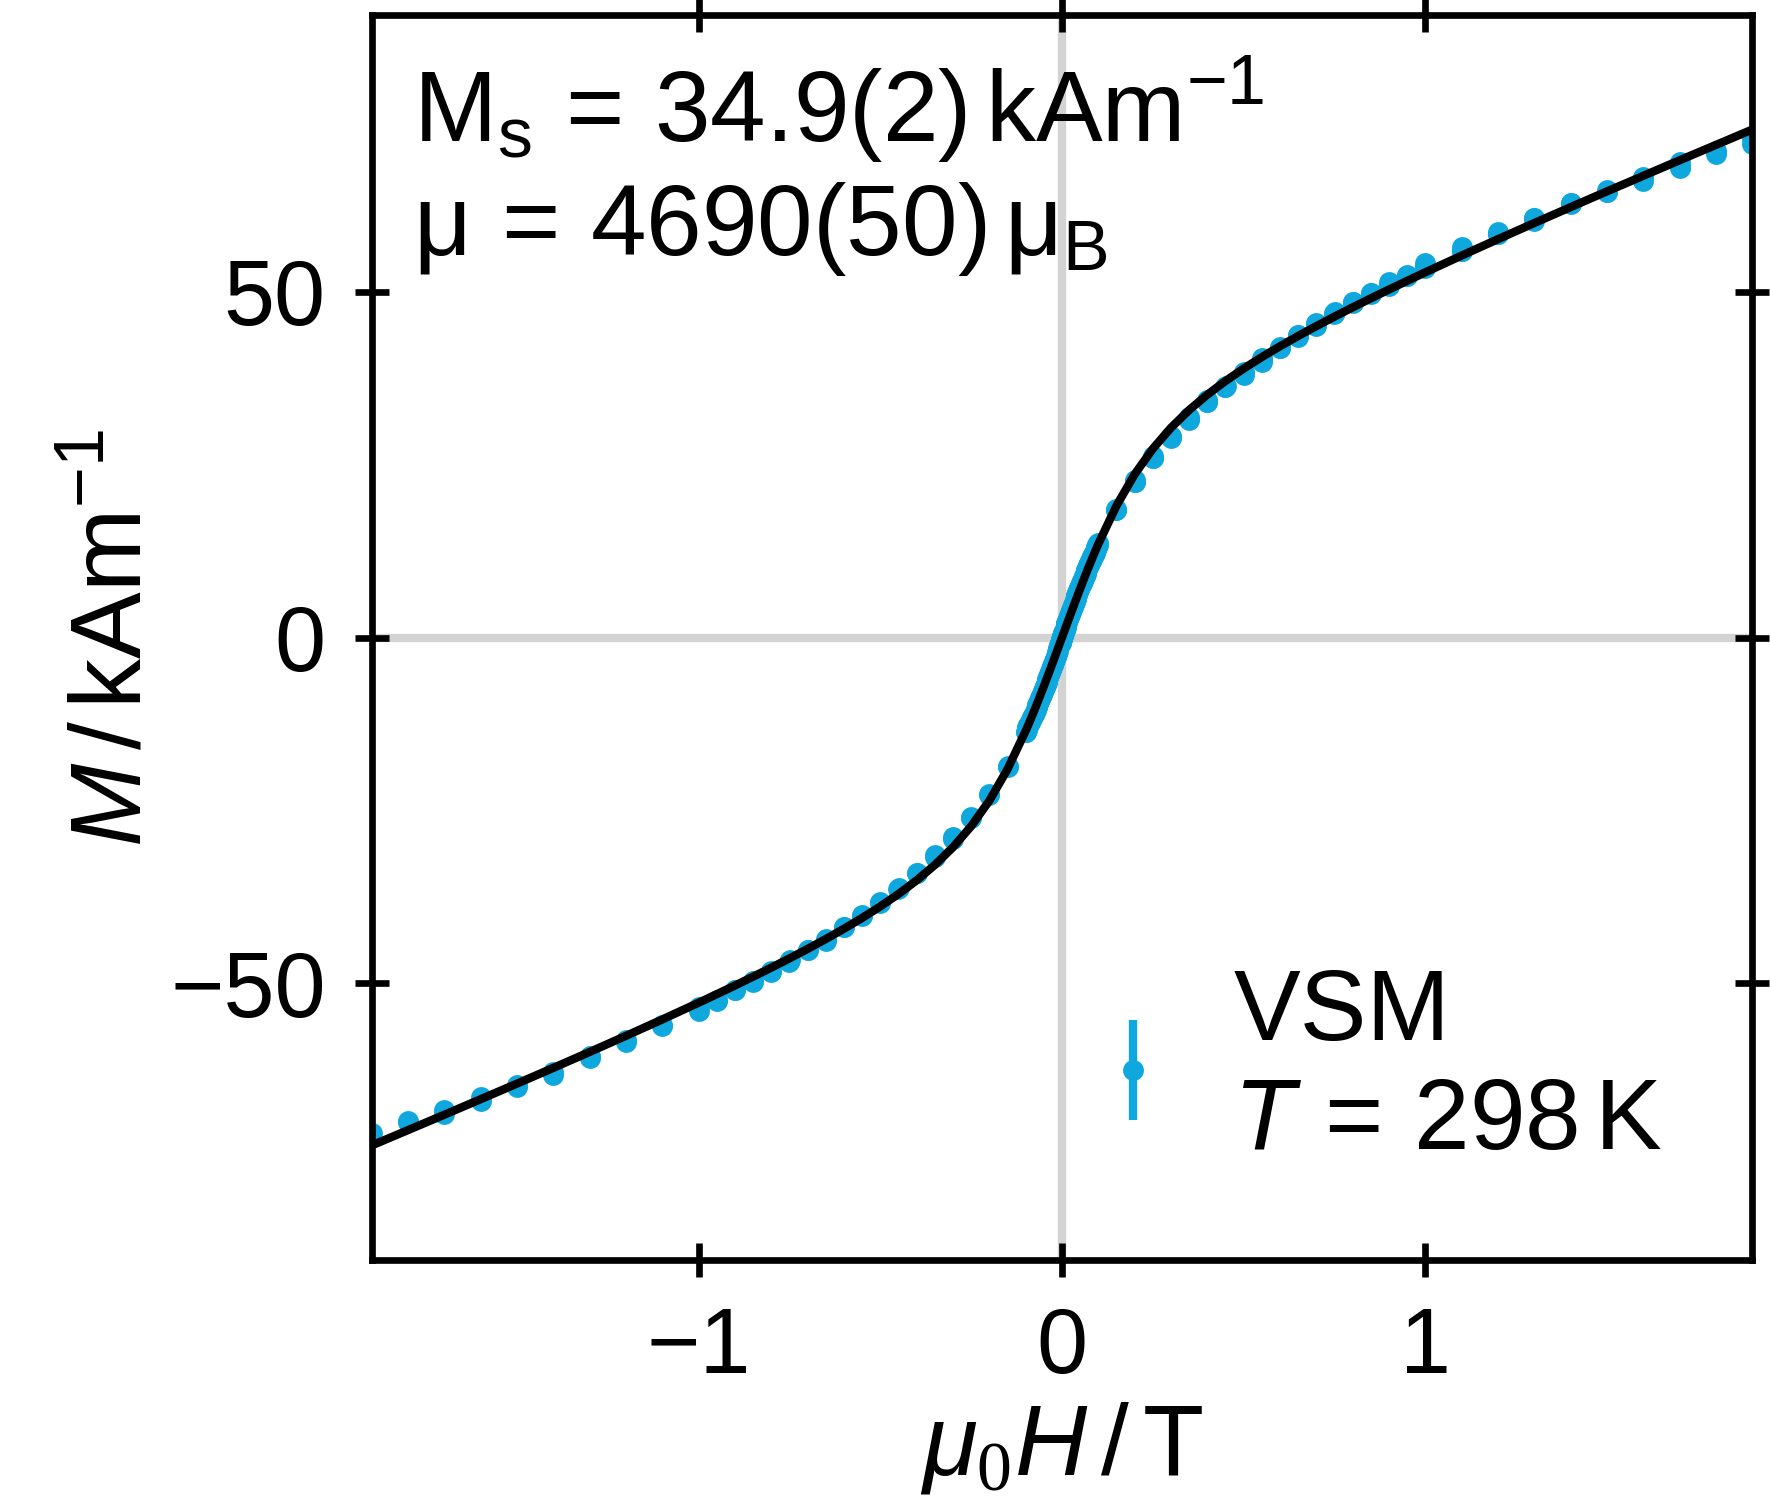
\includegraphics{monolayer_VSM_Ol_CoFe_C}
      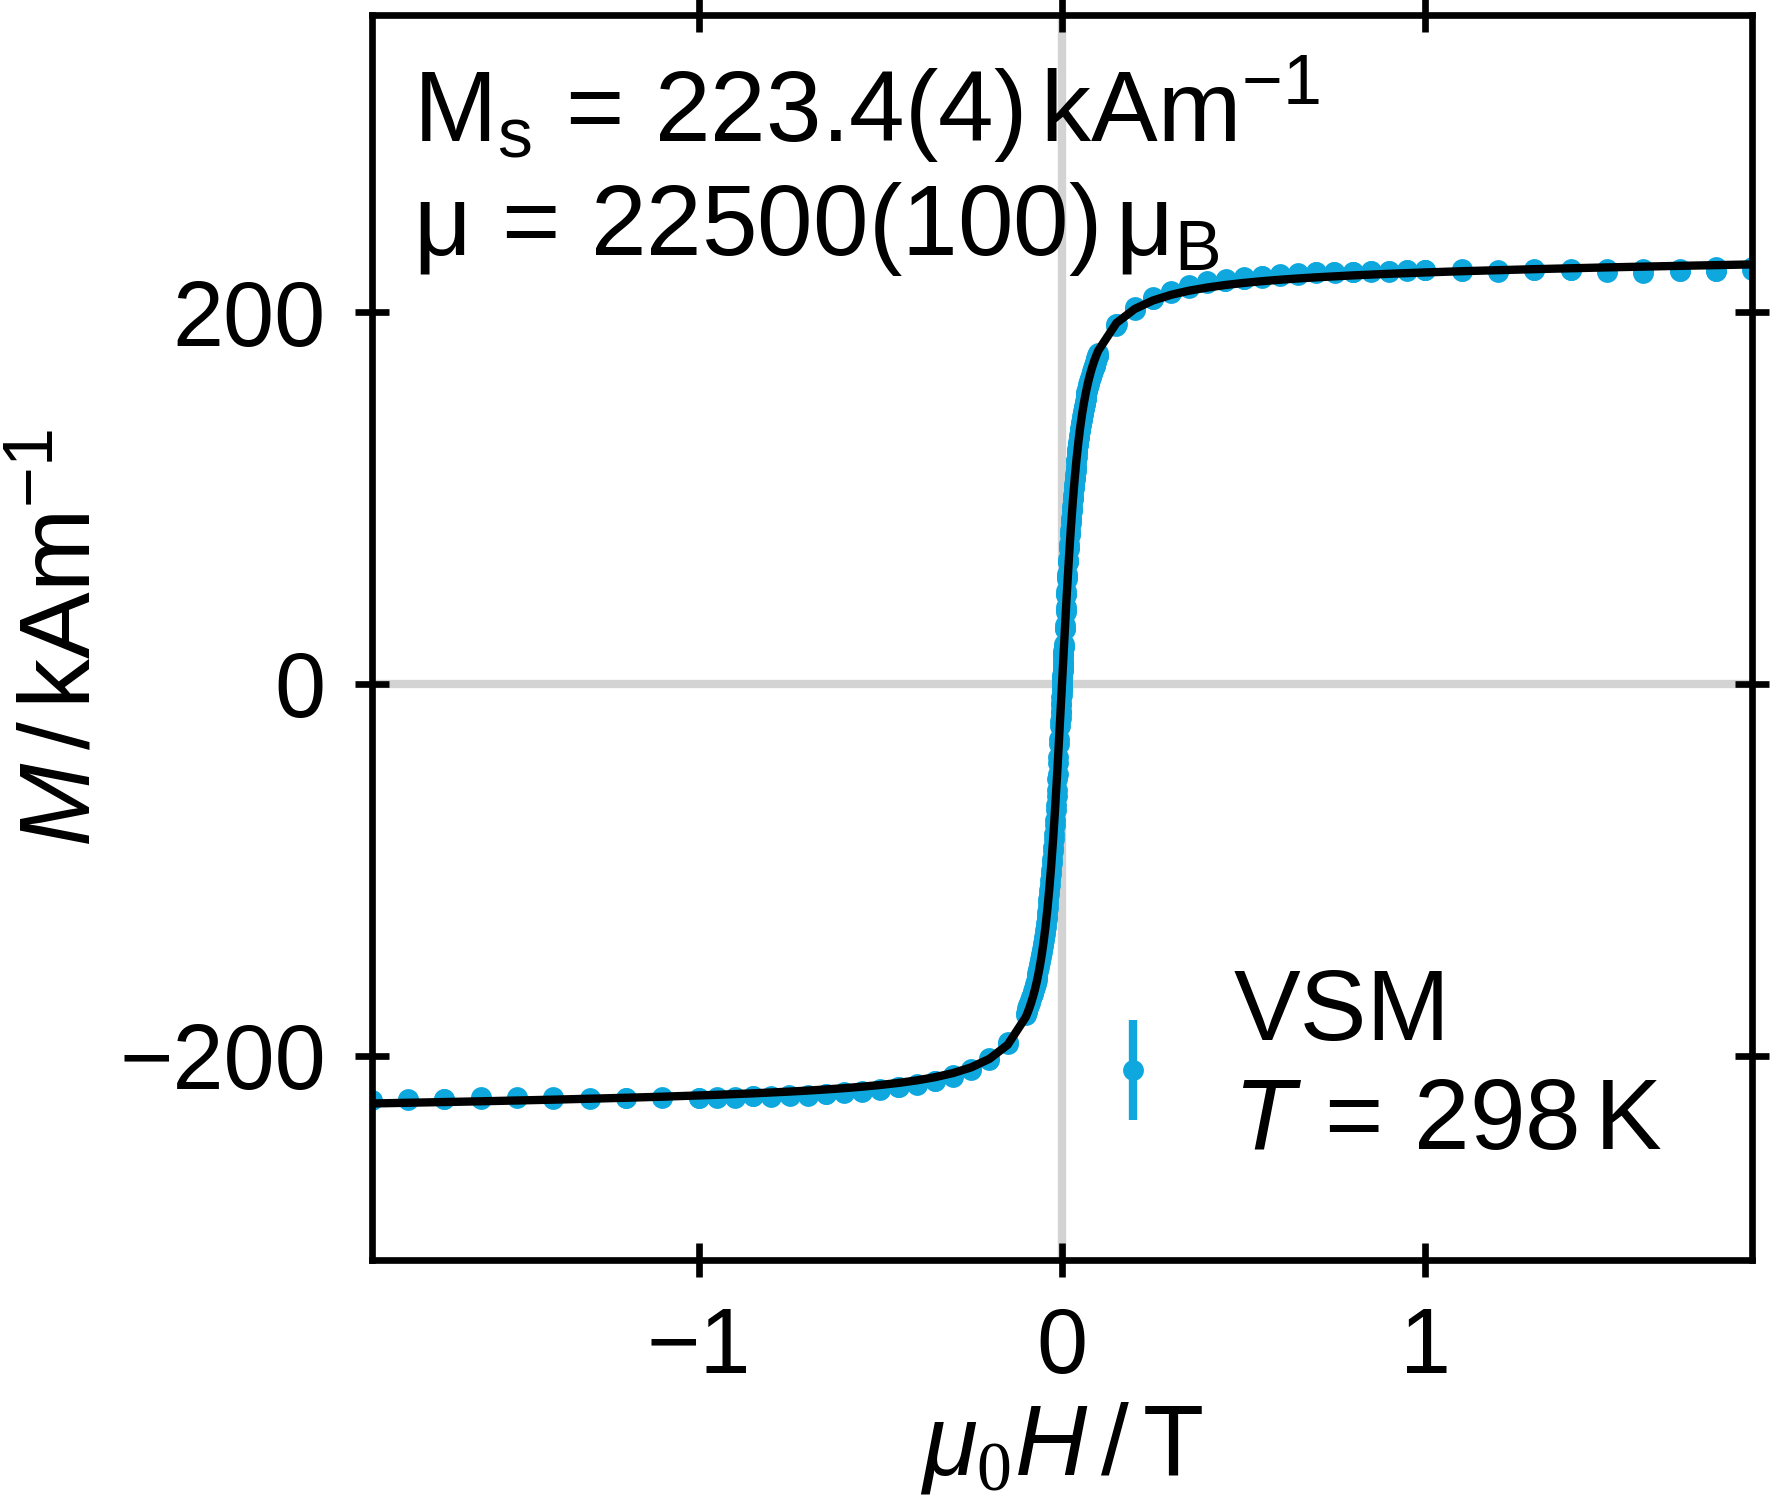
\includegraphics{monolayer_VSM_Ac_CoFe_C}
      \caption{\label{fig:monolayers:nanoparticle:vsm}Room-temperature VSM data of Ol-CoFe-C (upper left) and Ac-CoFe-C (lower left) dried on a substrate and fitted to a Langevin curve.}
    \end{figure}

    This can be compared to the magnetization obtained from measuring the nanoparticles on a vibrating sample magnetometer (VSM) as shown in \reffig{fig:monolayers:nanoparticle:vsm}, which results in magnetizations of $57 \unit{kAm^{-1}}$ for Ol-CoFe-C and $149 \unit{kAm^{-1}}$ for Ac-CoFe-C at the same magnetic field of $1.2 \unit{T}$.

    Both experiments agree in the result that the nanoparticles from the oleate route are weakly magnetic, while the particles from the acetylacetonates are stronger magnetic.

  \paragraphNewLine{Temperature-Dependant VSM}
  \begin{figure}[tb]
    \centering
    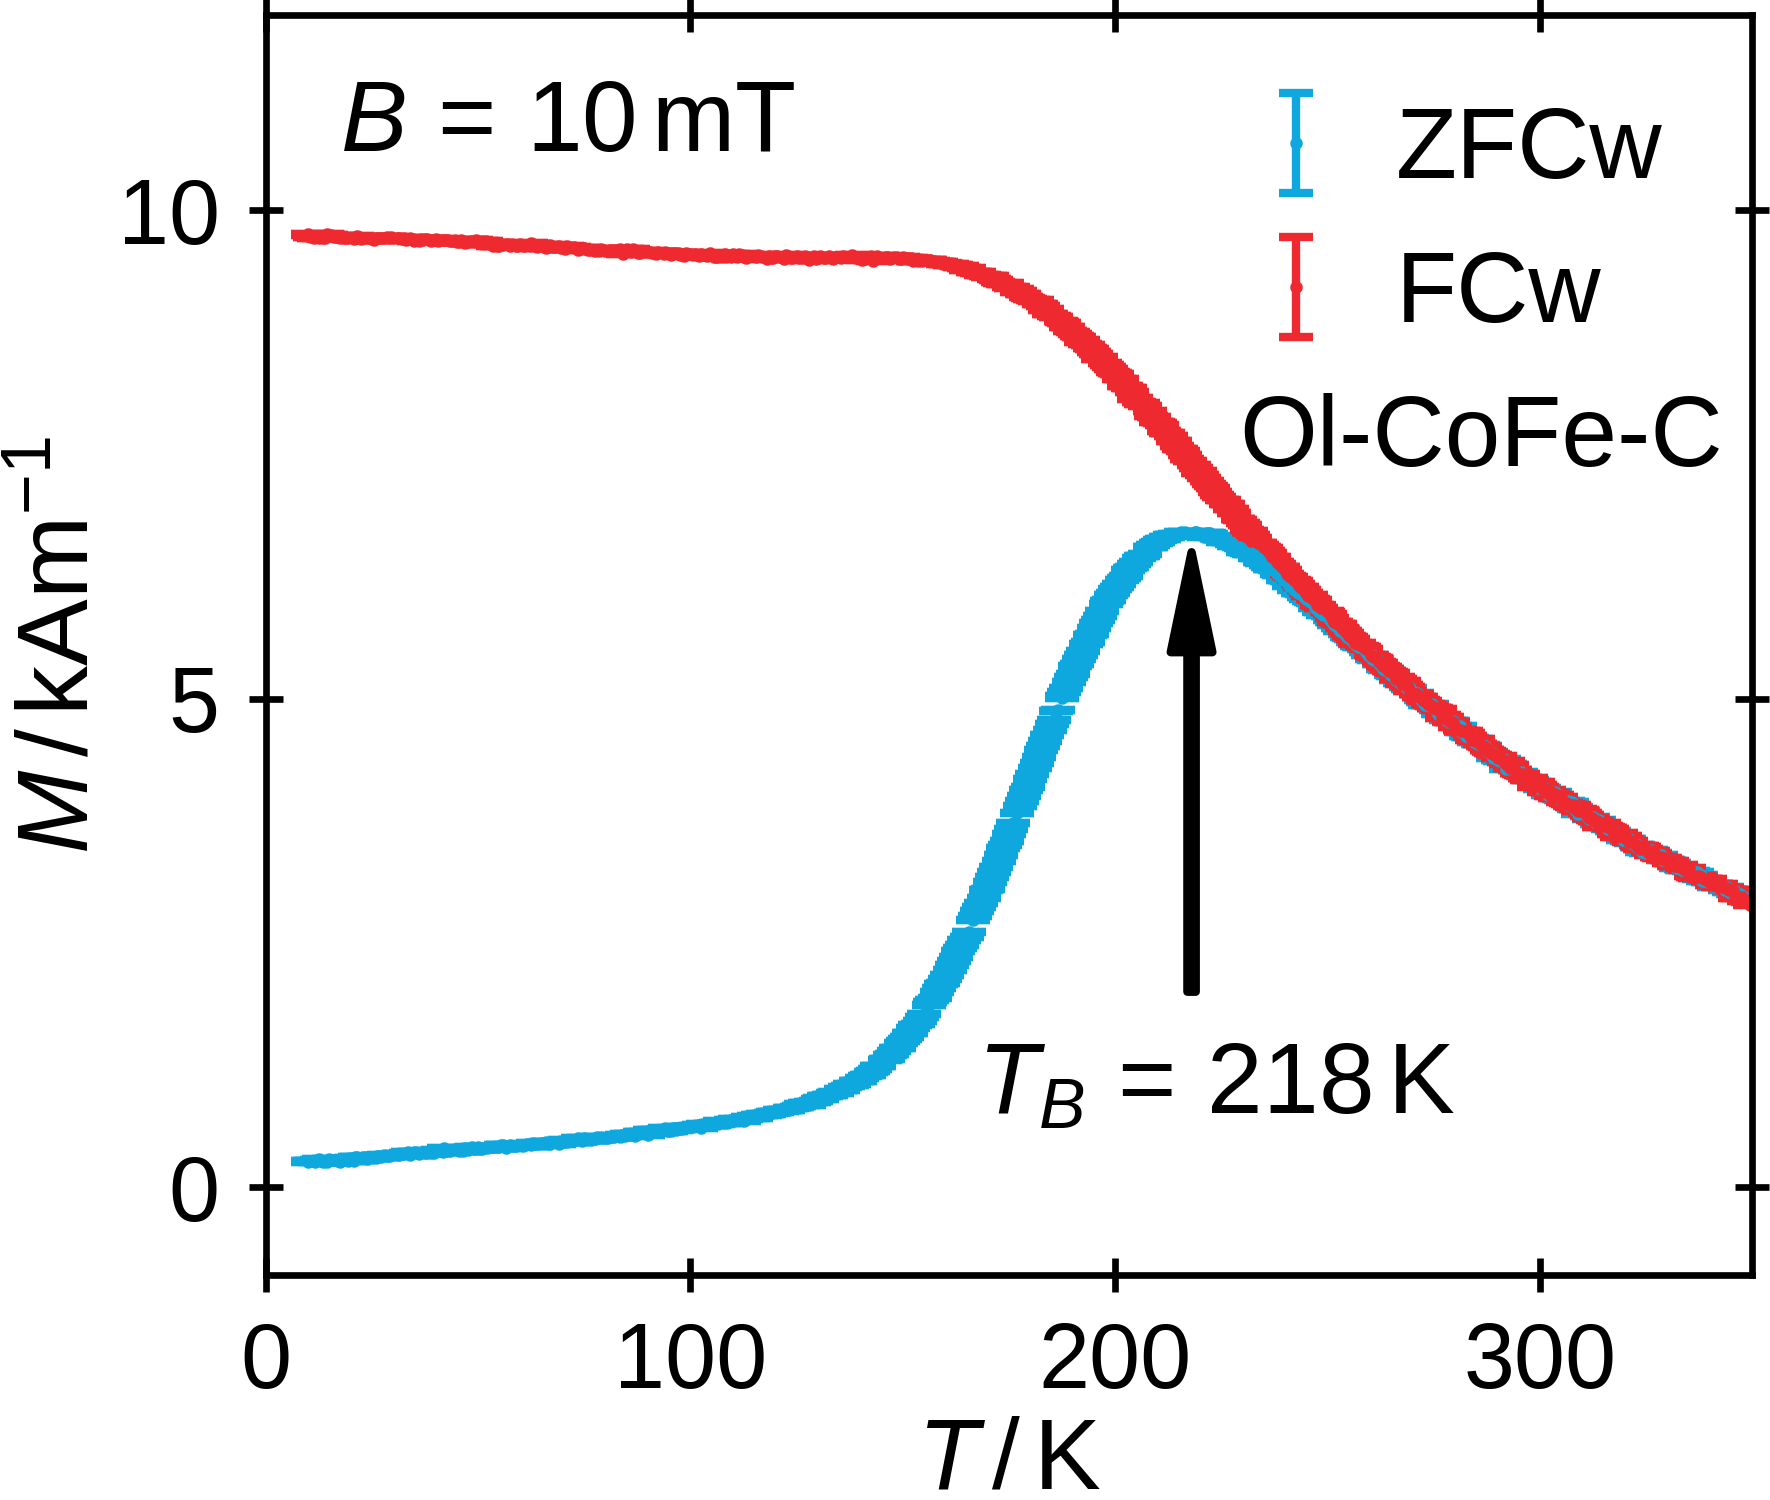
\includegraphics{monolayer_PPMS_ZFC_FC_ML_Ol_CoFe_C}
    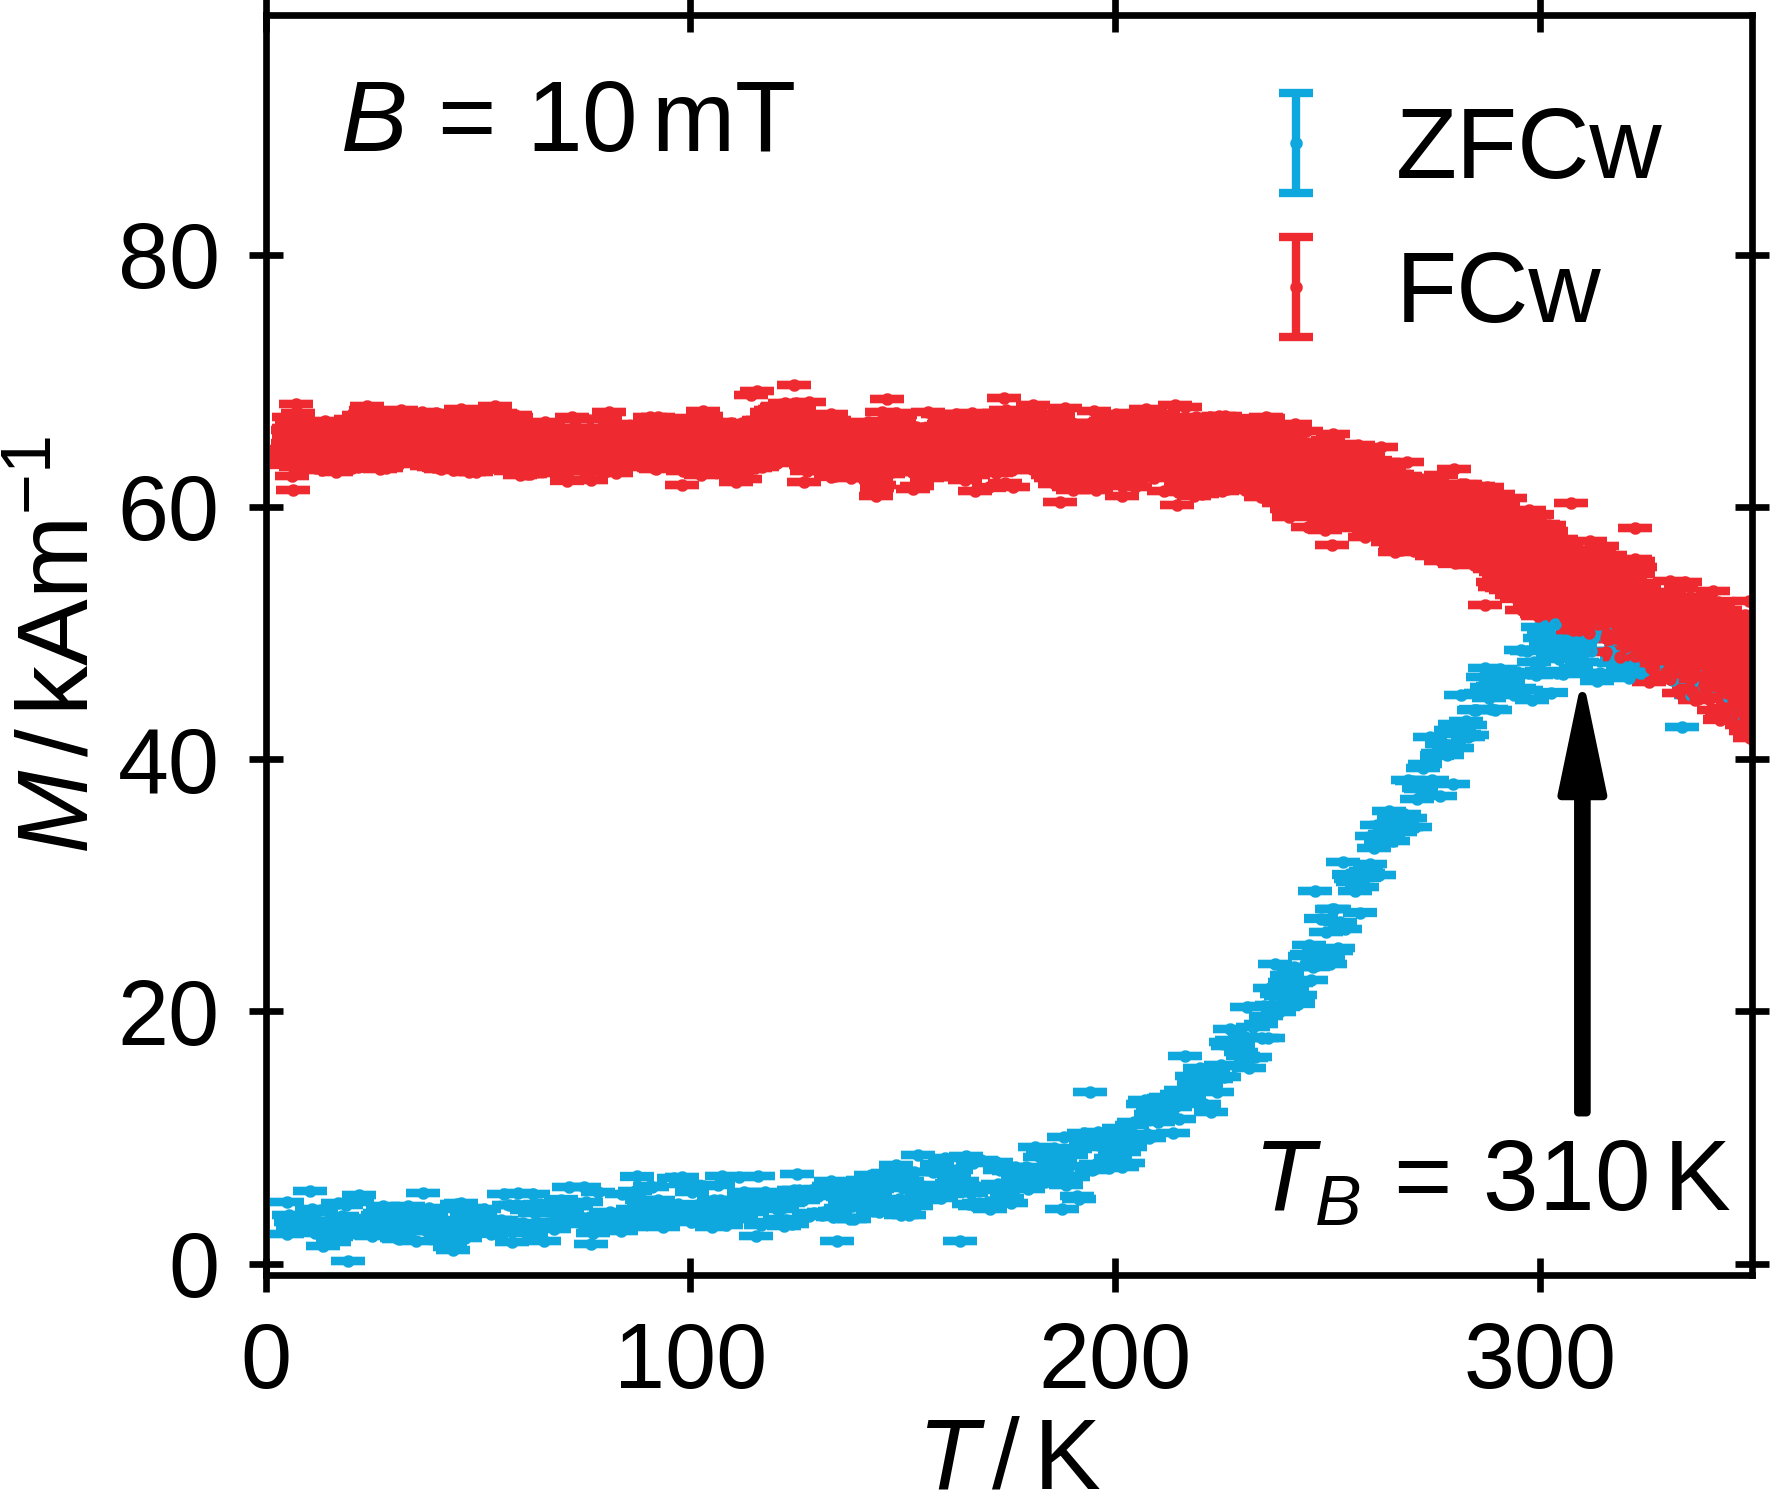
\includegraphics{monolayer_PPMS_ZFC_FC_ML_Ac_CoFe_C}
    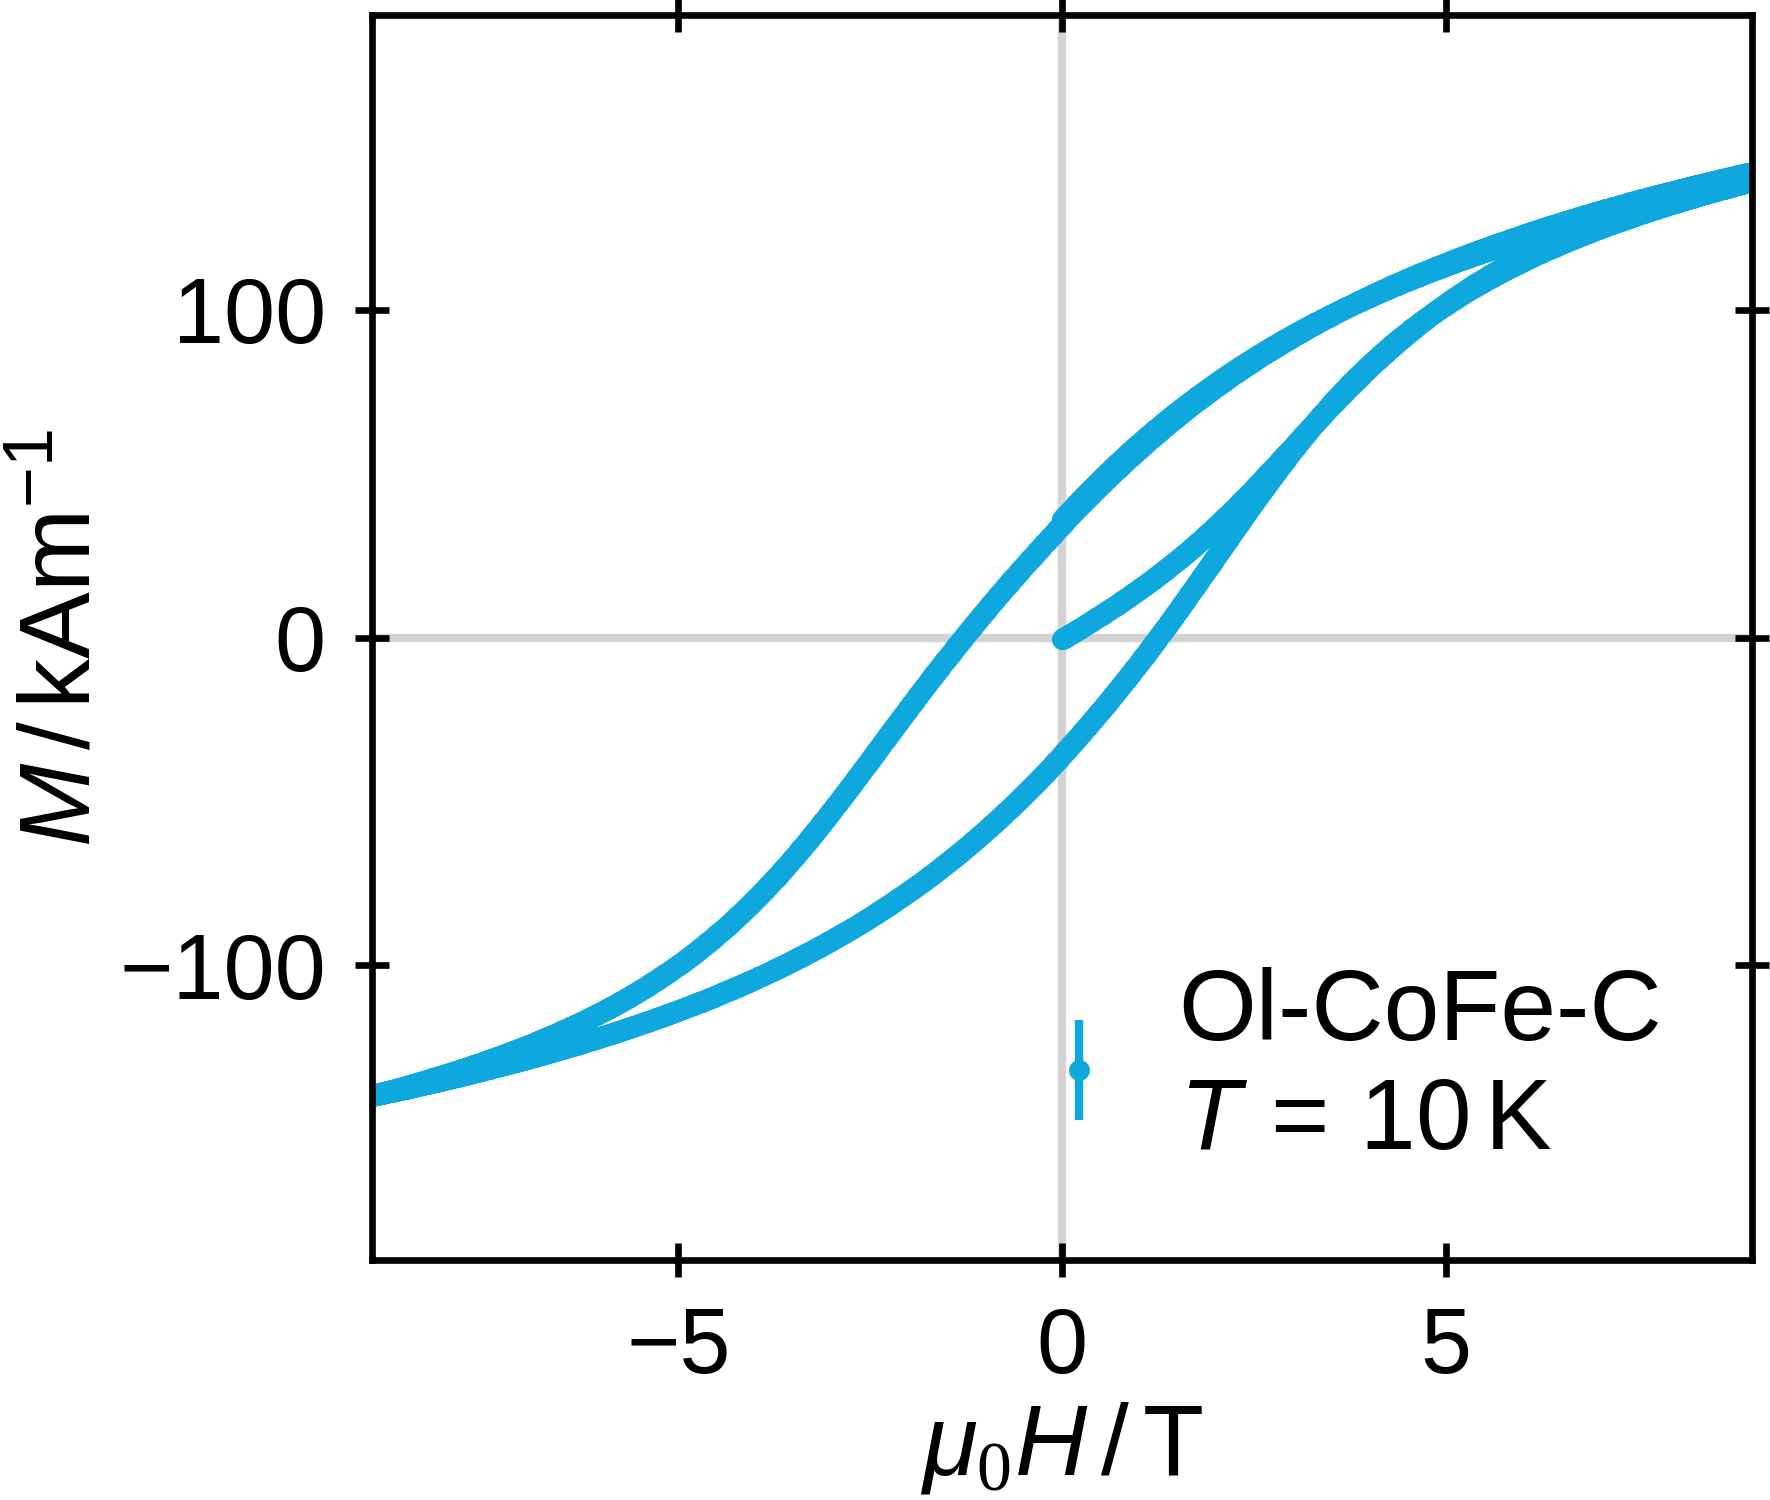
\includegraphics{monolayer_VSM_10K_Ol_CoFe_C}
    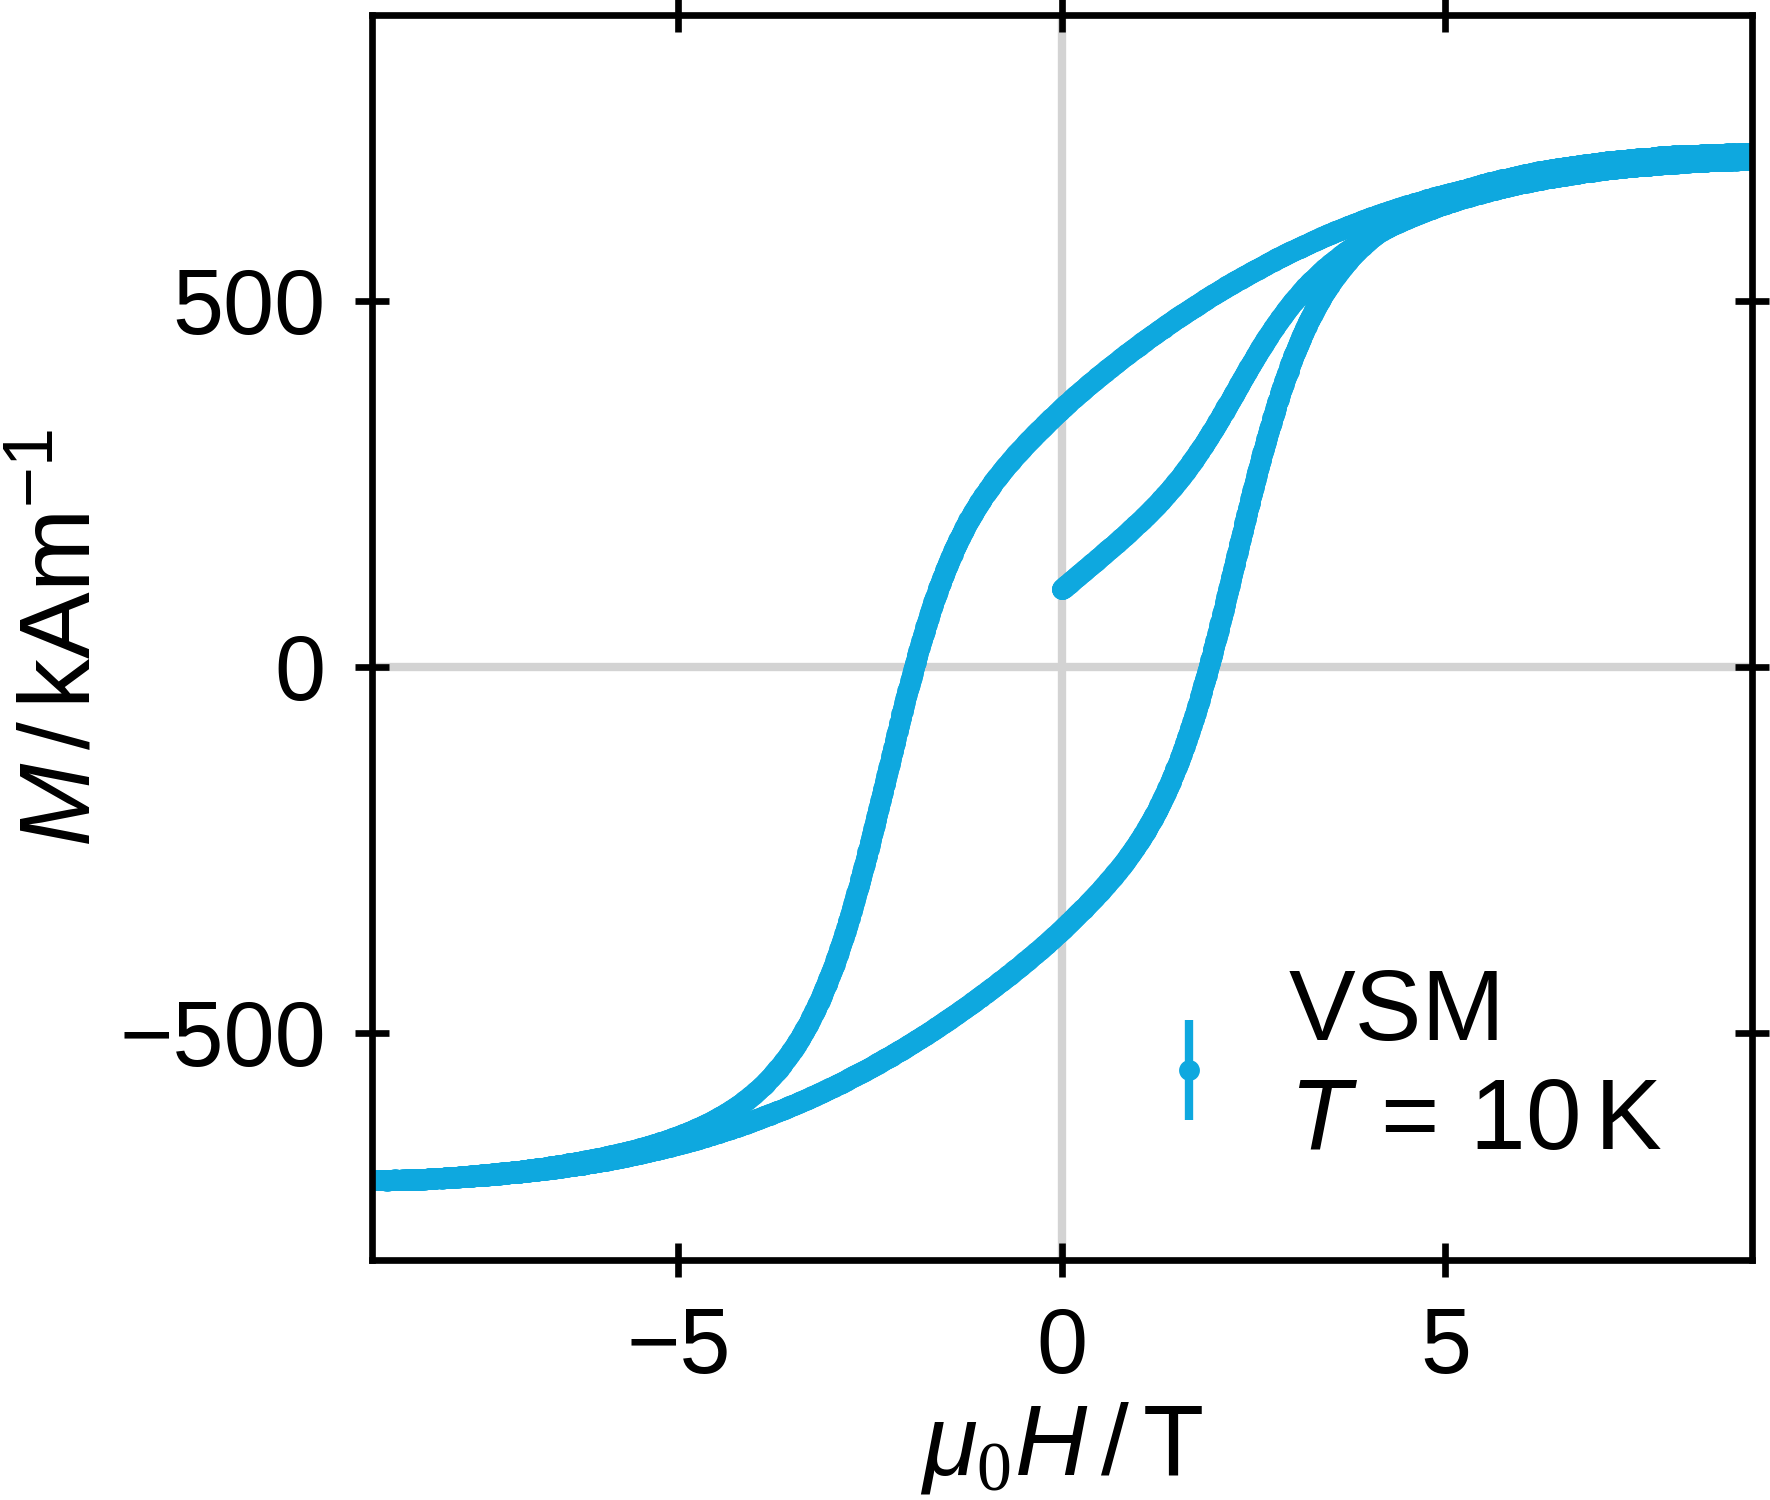
\includegraphics{monolayer_VSM_10K_Ac_CoFe_C}
    \caption{\label{fig:monolayers:nanoparticle:vsm10K}Low temperature hysteresis measurement of frozen Ol-CoFe-C (left) and Ac-CoFe-C (right) using the same samples as in \reffig{fig:monolayers:nanoparticle:vsm}.}
  \end{figure}
\end{document}